\section{Constant Value}
Some non-lethal obstacles are defined by constant values, such as the interaction areas of \citet{fraichard:anthronav} or the perimeter of the parking lot in \citet{likhachev:costmaps}. This corresponds with 
\begin{displaymath}
   f(x, y) = \left\{
     \begin{array}{lr}
       A & : (x,y) \in Q\\
       0 & : (x,y) \notin Q
     \end{array}
   \right.
\end{displaymath}
that is to say, some constant value $A$ if the cell is in some subset of cells in the costmap. 

\begin{figure}[!t]
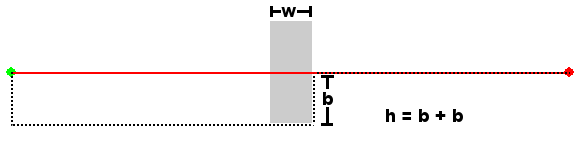
\includegraphics[width=\columnwidth]{graphix/Constant.png}
\caption{Two Paths with a Constant Non-lethal obstacle}
\label{fig:constant}
\end{figure}

If the subset of cells corresponds to all of the cells in some bounding box between the start and goal, then there are essentially only two feasible paths as seen in Figure \ref{fig:constant}. The first (solid red in the figure) is the straight path through the obstacle which has a cost of 
\[ \Phi(p_1) = 2nP + \sum_{x=x_0}^{x_1} f(x, 0) \]
or, if we define the width of the obstacle to be $w$, 
\[ \Phi(p_1) = 2nP + wA \]

The other path (shown in a dotted black line in the figure) avoids the obstacle entirely, taking the shortest path around the obstacle, which is longer than $p_1$ by some constant $d$. Thus, the cost is
\[ \Phi(p_2) = (2n + d)P \]

Which of these two paths is the path less traveled depends on the values of $P$, $wA$ and $d$. To find when we take $p_1$, we consider the inequality 
\begin{align}
\Phi(p_1) < & \Phi(p_2)\notag\\
2nP + wA < & (2n + d)P \notag\\
wA < & dP 
\end{align}

Hence, we can force a planner to chose the straight path ($p_1$) by lowering the constant cost, decreasing the distance the path is within the obstacle, or by increasing the path constant or the length of the alternative path. This follows our intuition in this simple case, but we now also have a formula for computing proper parameters depending on the desired behavior, such that we can set up parameters where the switch between the two paths happens when the second path is precisely 15 cells longer, for example. 

There are other scenarios you could construct with constant valued obstacles, and many of them follow the same sort of logic shown here but with more cases and mildly more complex math. The authors encourage others to work through the math as the specific scenarios arise. 




